\chapter{\ChapterTitleScope}
\label{sec:zakres-funkcjonalnosci}


\section{Kontekst użytkowania aplikacji}

\begin{figure}[b!]
  \centering
  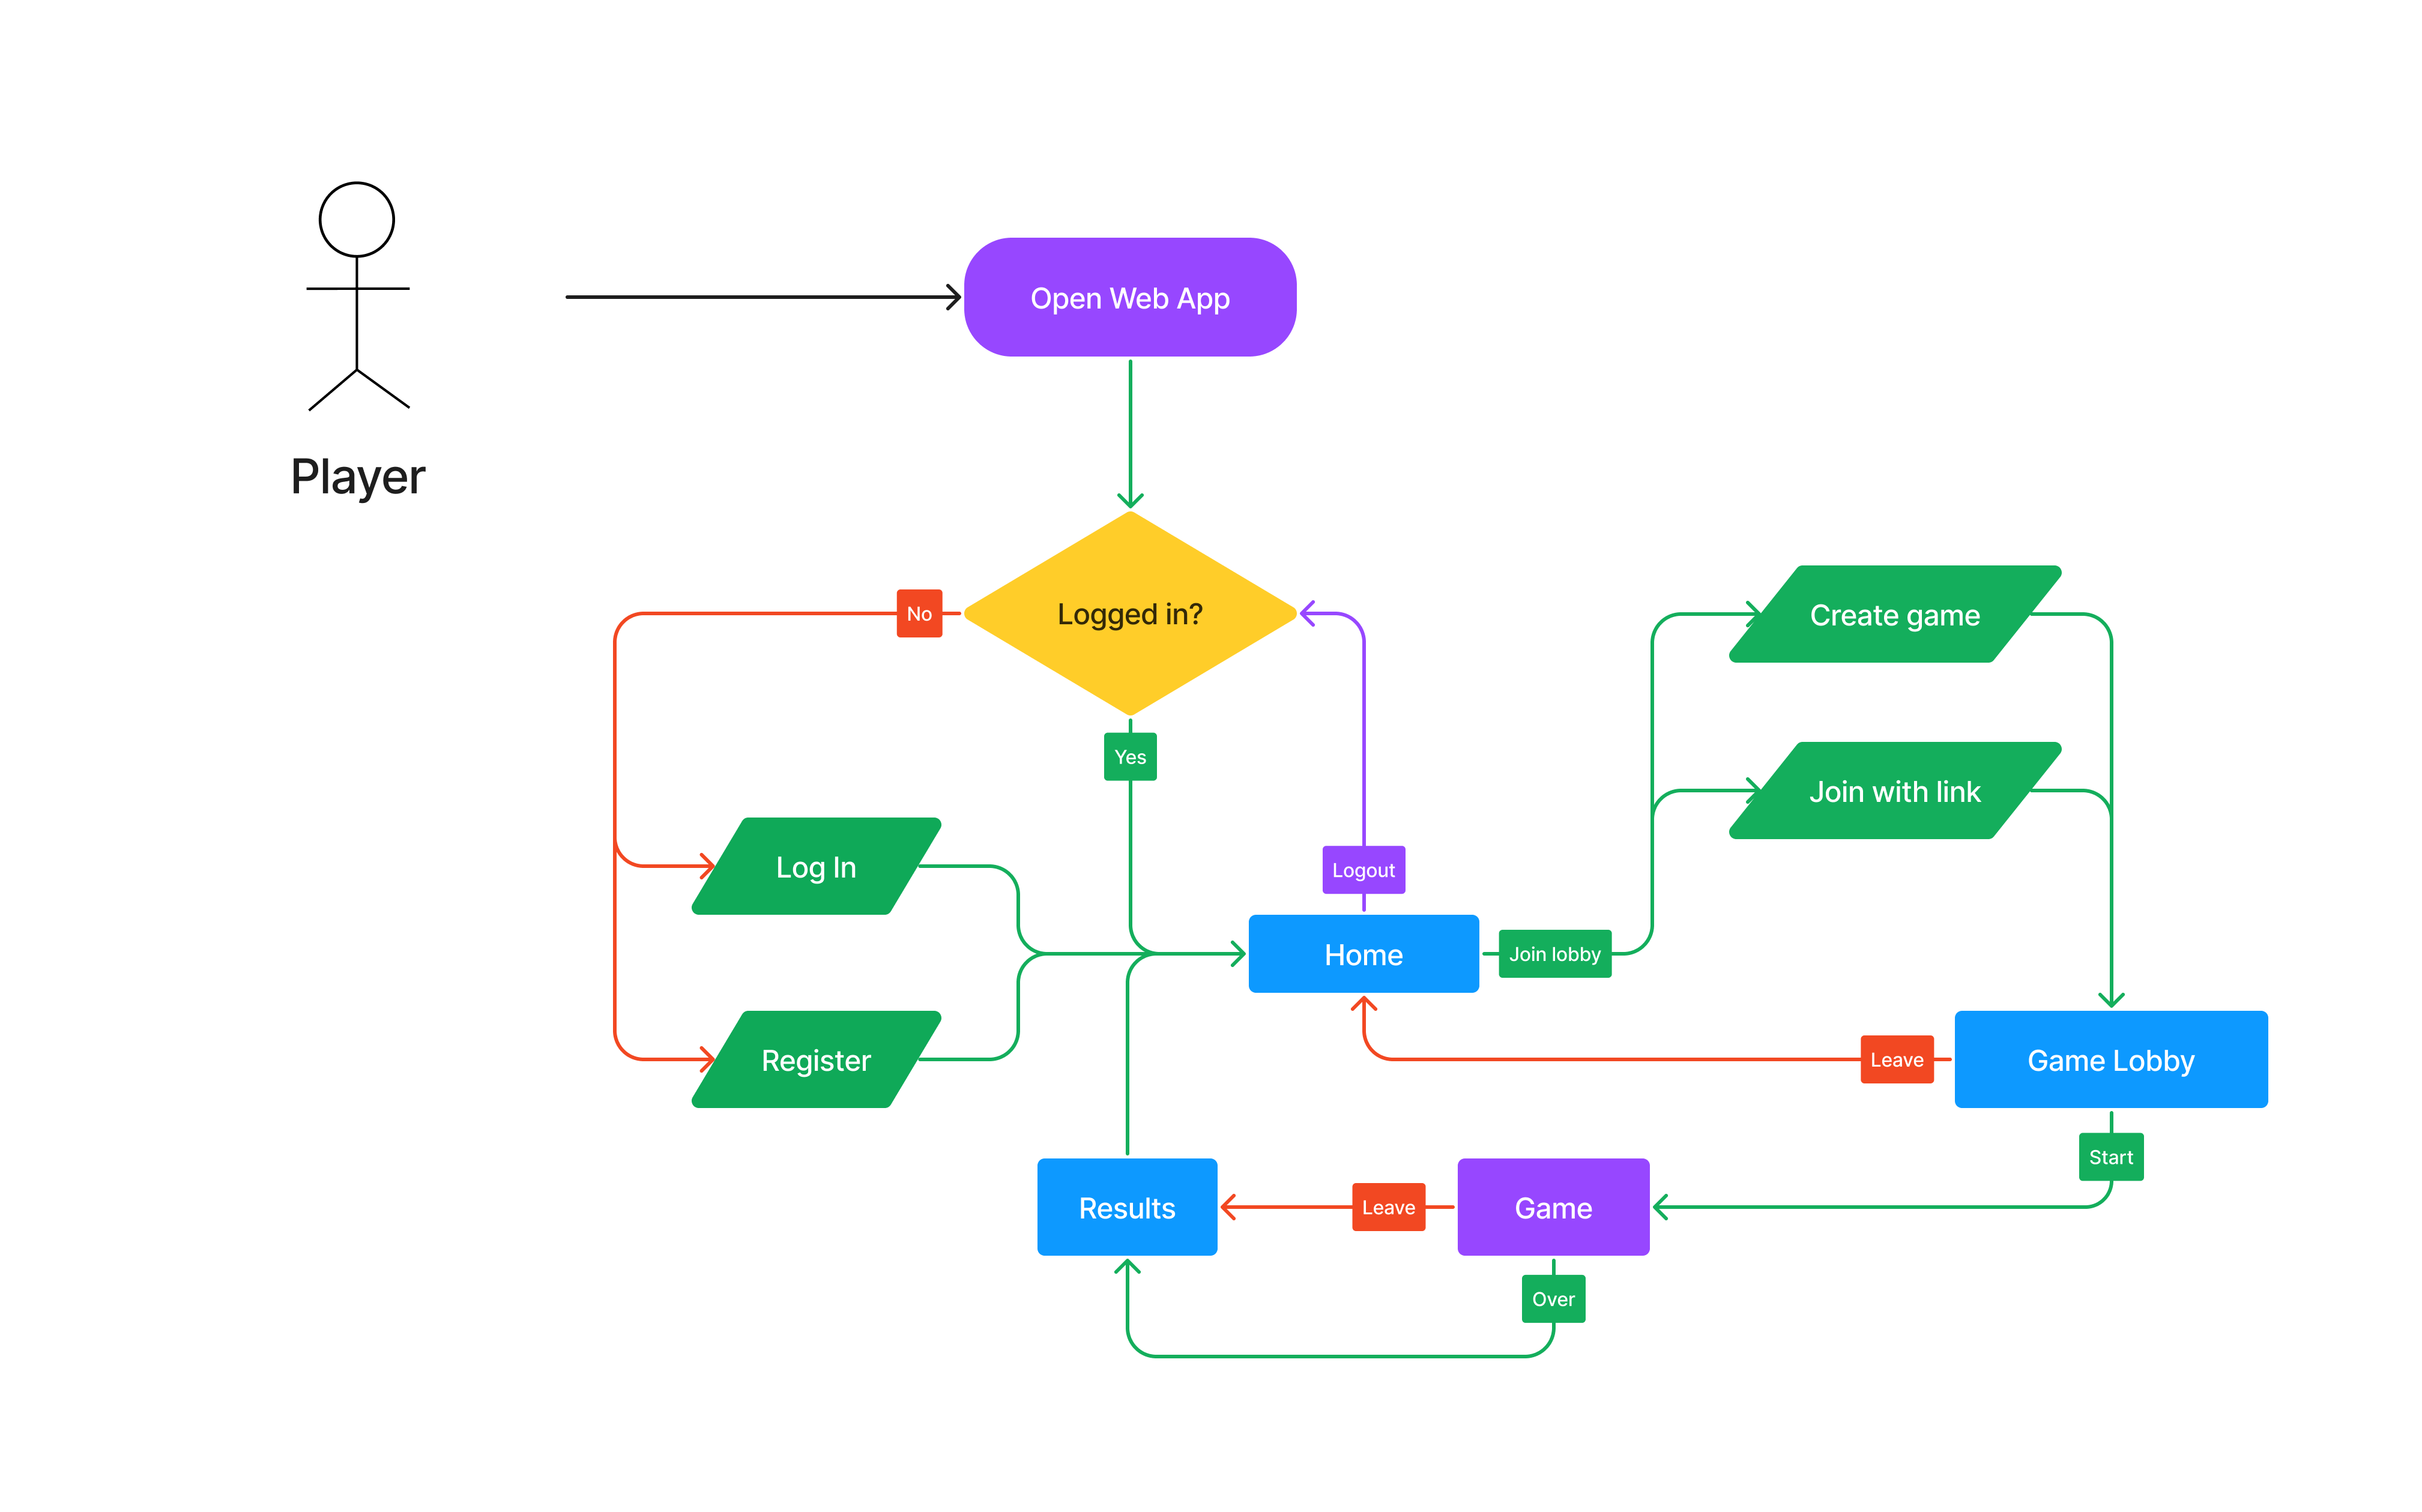
\includegraphics[width=0.9\textwidth]{img/flow-aplikacji/user_flow.png}
  \caption{Schemat interakcji użytkownika z aplikacją}
  \label{fig:figma_userflow}
\end{figure}

\begin{figure}[p!]
  \centering
  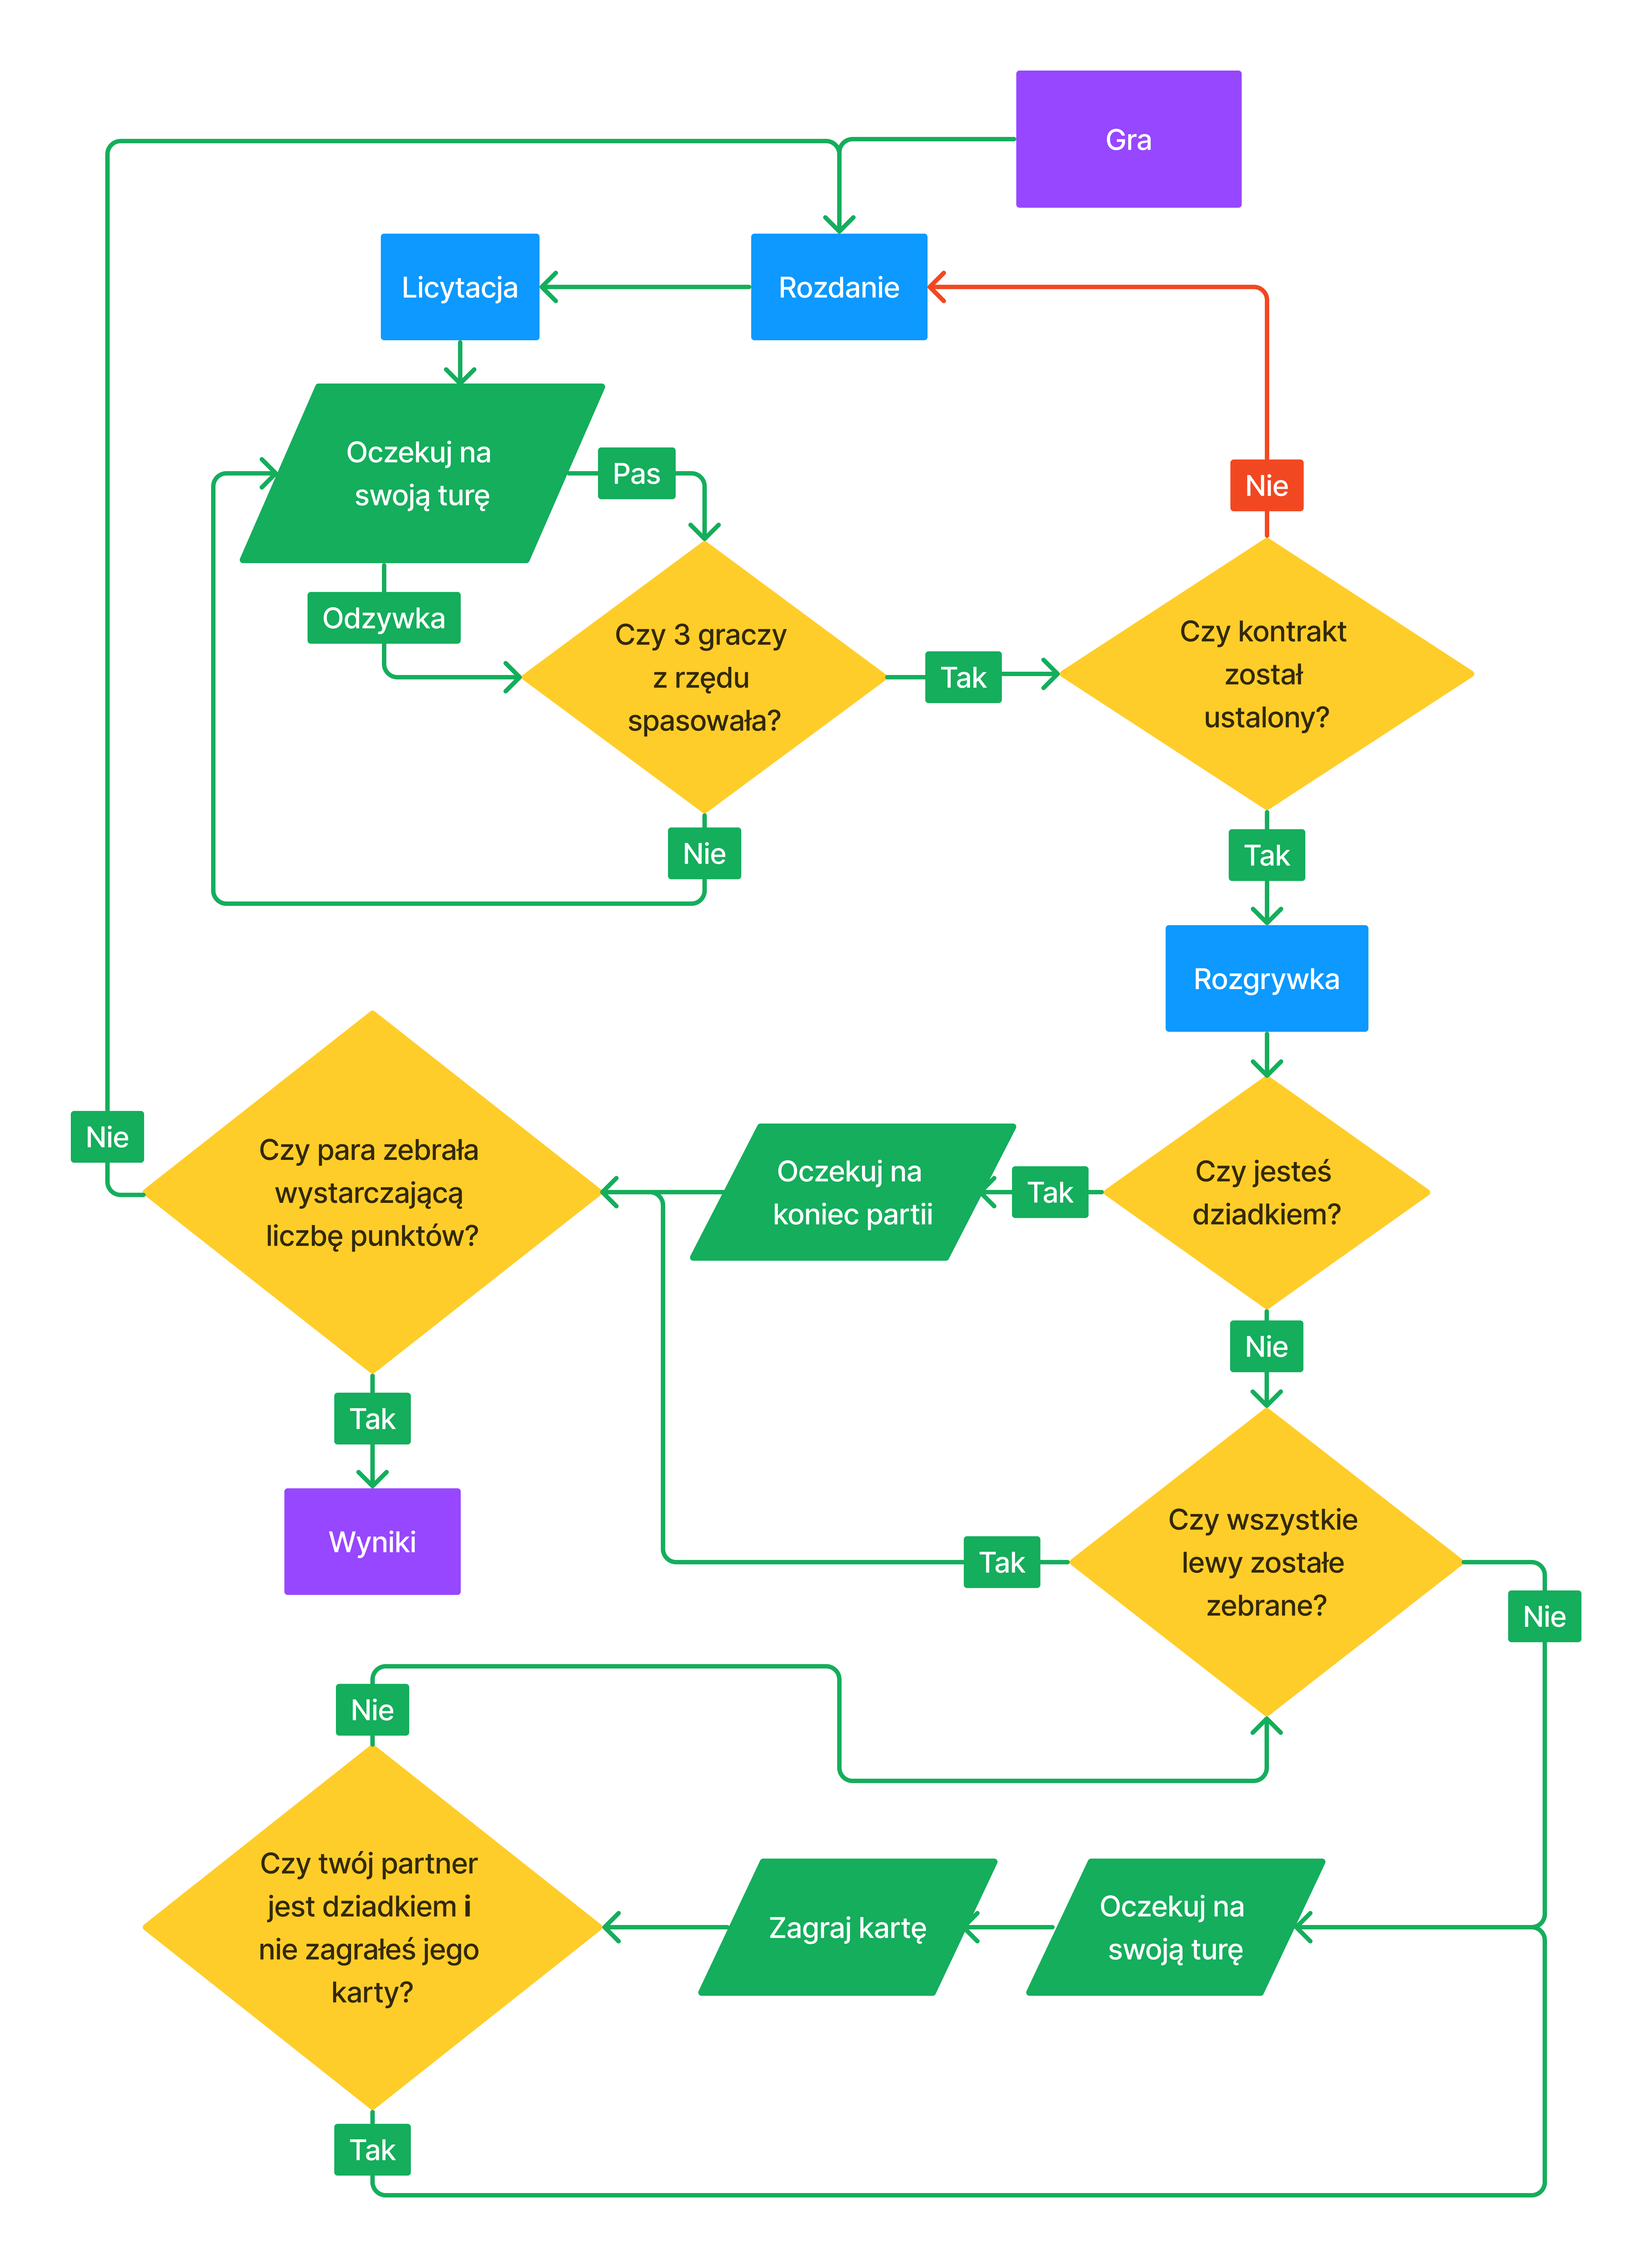
\includegraphics[width=\textwidth]{img/flow-aplikacji/game_flow.png}
  \caption{Schemat interakcji użytkownika z aplikacją podczas rozgrywki brydża}
\end{figure}

Głównym zadaniem aplikacji jest oferowanie możliwości
rozgrywania gry w~brydża. Strona internetowa aplikacji ma być
przystosowana do dowolnego rozmiaru ekranu urządzenia, z~którego mógłby
korzystać użytkownik. Dzięki temu można skorzystać z~aplikacji, wykorzystując
telefon, komputer stacjonarny, laptop lub nawet telewizor. Wymagany
jest tylko dostęp do Internetu. \\


W~systemie aplikacji zdefiniowane są dwa typy użytkowników:
\begin{itemize}
  \item \textbf{anonimowy użytkownik} -- osoba niezalogowana, która nie
        posiada dostępu do funkcjonalności aplikacji związanych
        z~rozgrywką.

  \item \textbf{zalogowany użytkownik} -- zalogowana osoba posiadająca konto
        w~aplikacji, mająca pełny dostęp do jej funkcjonalności.
\end{itemize}

Funkcjonalności dostępne dla poszczególnych użytkowników:
\begin{itemize}
  \item \textbf{anonimowy użytkownik}:
        \begin{itemize}
          \item rejestracja nowego konta w~systemie aplikacji.
          \item logowanie do konta utworzonego w~systemie aplikacji.
        \end{itemize}

  \item \textbf{zalogowany użytkownik}:
        \begin{itemize}
          \item funkcjonalności użytkownika anonimowego.
          \item tworzenie i~dołączanie do rozgrywek w brydża --
                gdy użytkownik założy lub zostanie jedynym
                użytkownikiem lobby, to staje się jego
                hostem.
          \item zarządzanie lobby -- może decydować o~graczach znajdujących wraz
                z~nim w~lobby. Może decydować o~ich pozycji lub ich wyrzucić
                ze wspólnej sesji\footnote{Sesja oznacza to samo co lobby, czyli
                  abstrakcję łączącą wielu graczy i~asystentów w~obrębie jednej
                  rozgrywki}.
                Może także uzupełnić wolne miejsca o~asystenta brydża z~określeniem jego
                poziomu trudności.
        \end{itemize}
\end{itemize}

\FloatBarrier

\section{Przypadki użycia}

\subsection{Rejestracja i logowanie do aplikacji}

Aby uzyskać dostęp do większości funkcjonalności aplikacji, wymagane
jest posiadanie konta. Anonimowy użytkownik może je utworzyć, klikając
opcję \textbf{"Register"} w~nagłówku strony. Po kliknięciu użytkownik
zostanie przekierowany do formularza rejestracyjnego.
Do utworzenia konta wymagane jest podanie własnego
pseudonimu, adresu e-mail oraz hasła. Aby uzyskać dostęp do utworzonego
konta, należy kliknąć \textbf{"Log in"} w~nagłówku strony, po czym
w~formularzu podać dane wykorzystanie podczas rejestracji.

\begin{figure}[hbt!]
  \centering
  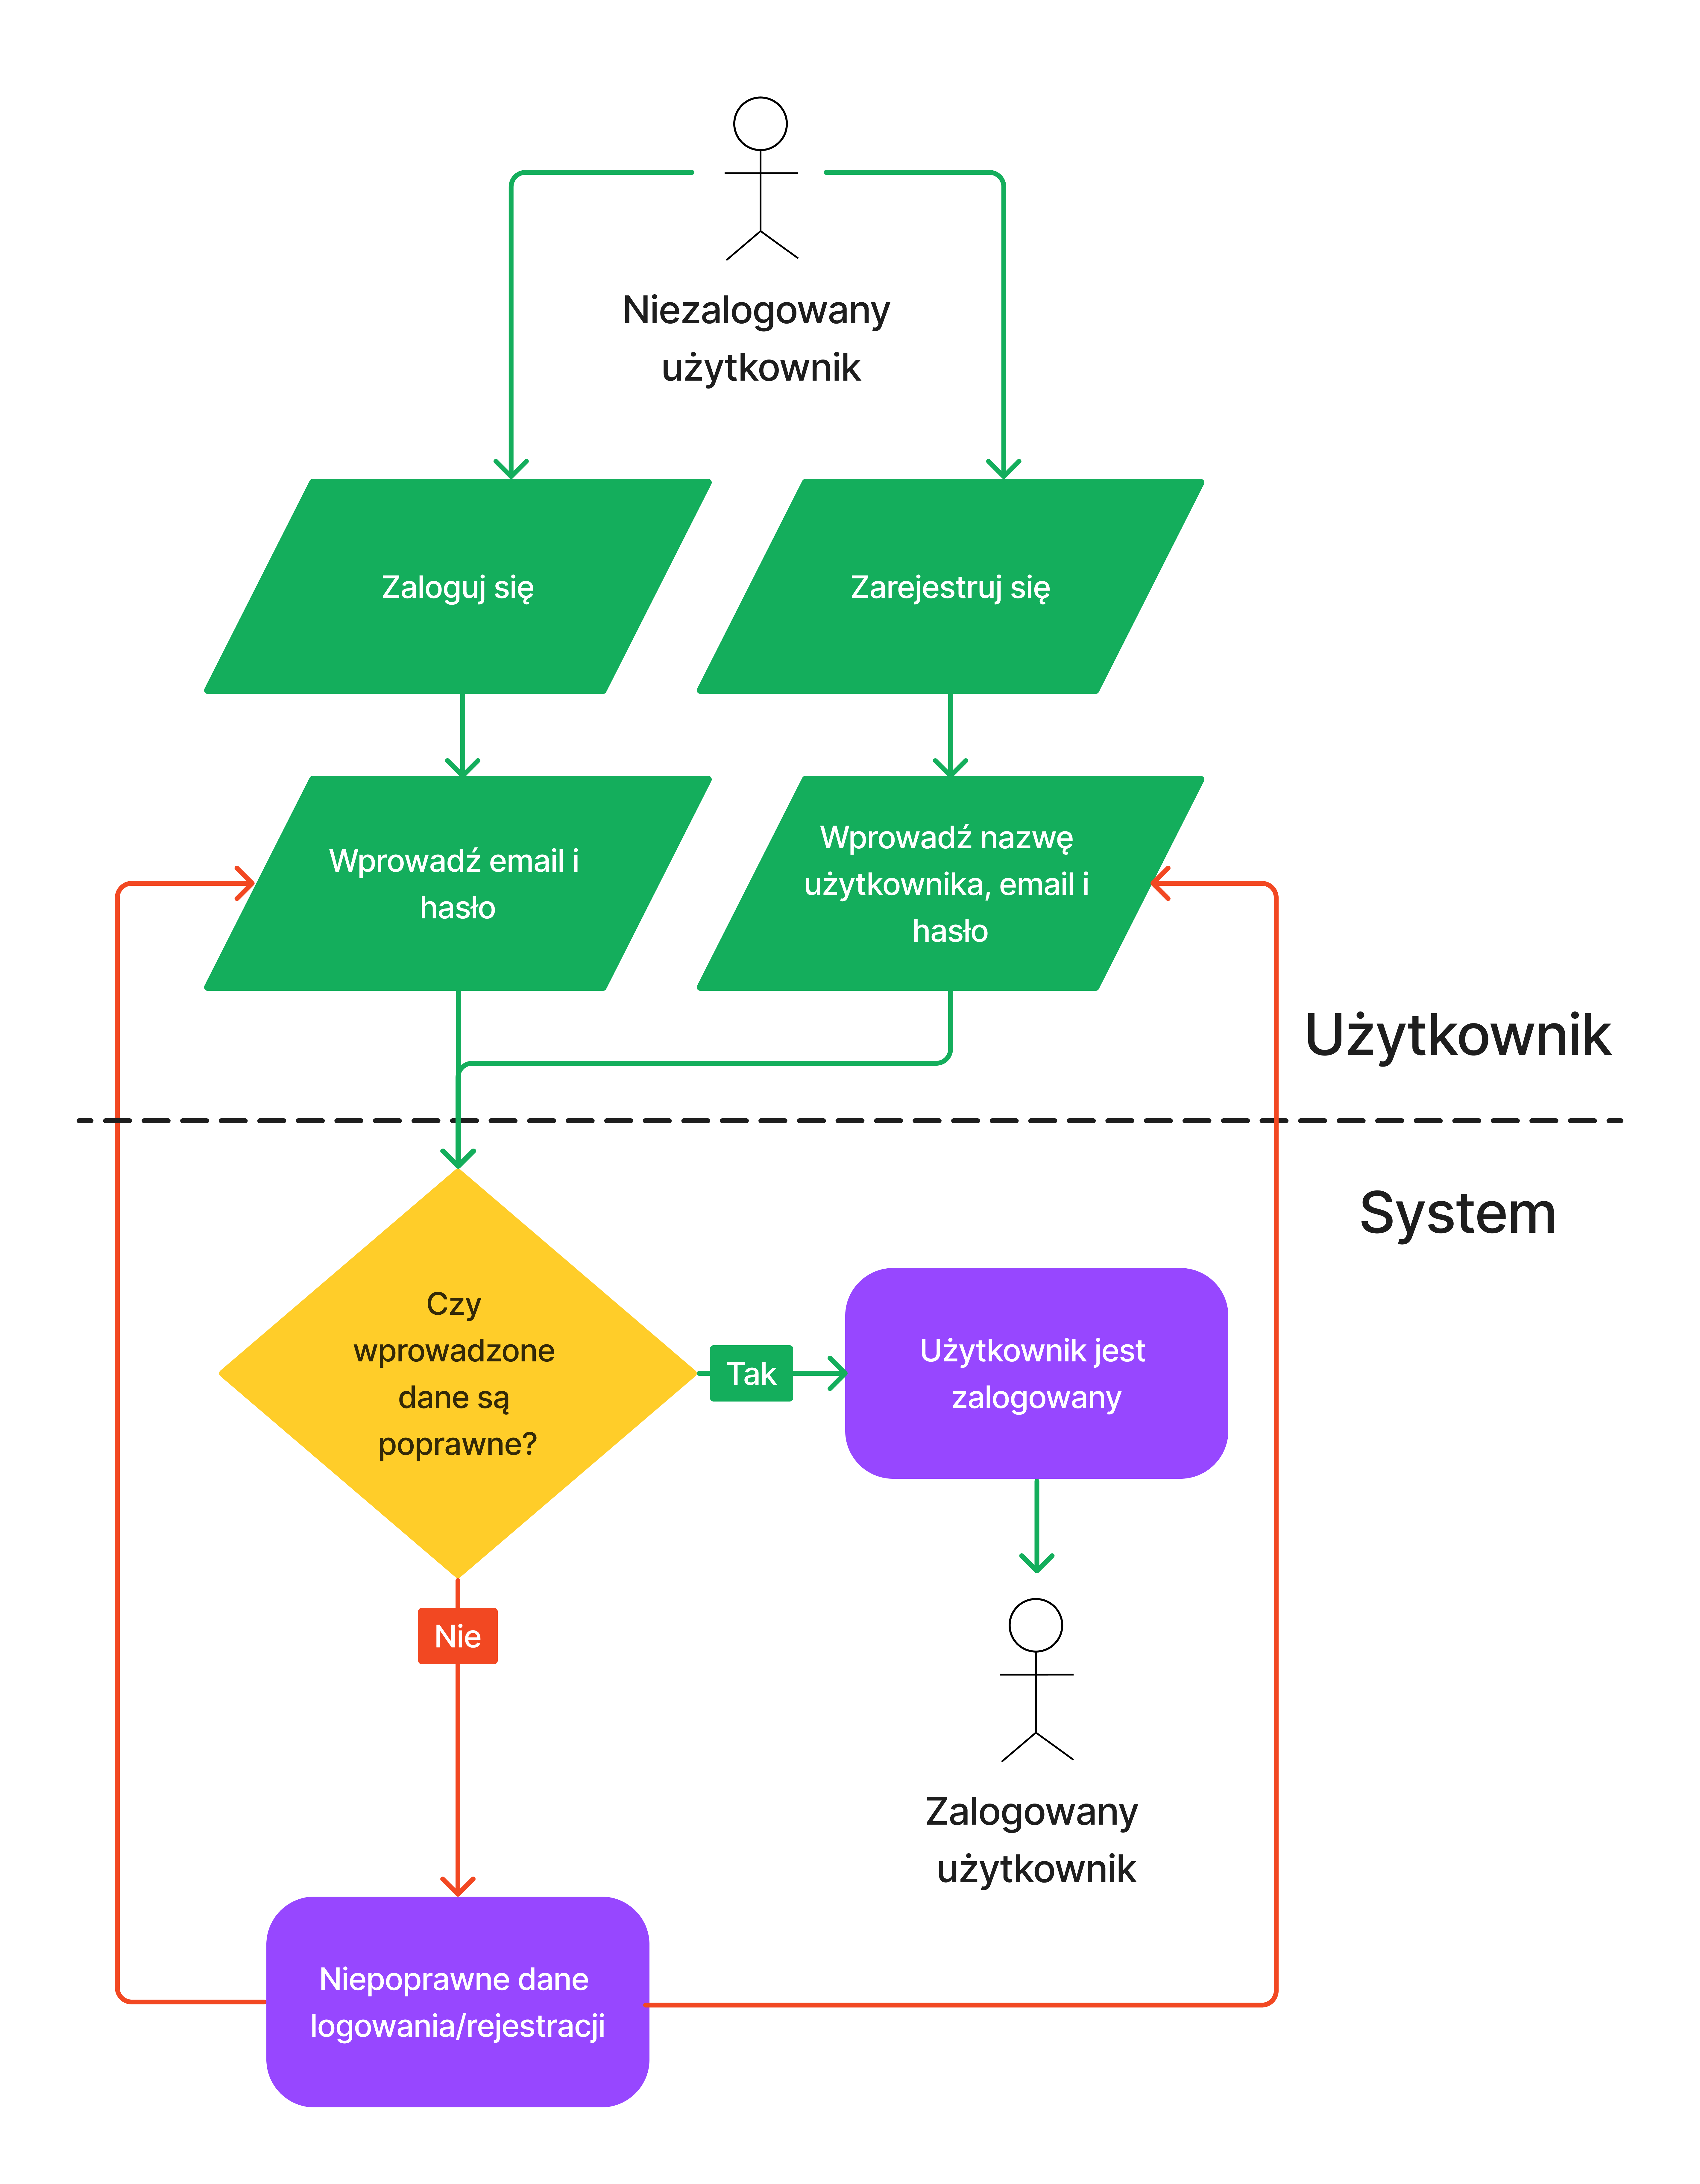
\includegraphics[width=0.9\textwidth]{img/schematy/login.png}
  \caption{Schemat logowania i~rejestracji użytkownika}
\end{figure}

W~przypadku nieprawidłowo podanych danych podczas rejestracji
lub logowania, wystąpienia błędów wynikających z~połączenia internetowego lub
niedostępnego serwerem autentykacji, użytkownik otrzyma odpowiednią
informację na ekranie.

\FloatBarrier


\subsection{Lobby}

\subsubsection{Tworzenie lobby}

Rozpoczęcie gry w~brydża jest dostępne z~poziomu lobby. Aby utworzyć
lobby, należy kliknąć \textbf{"Create lobby"} na głównym panelu
aplikacji. Przekieruje ono użytkownika do nowego lobby, którego staje
się administratorem. Do utworzonego lobby zostanie wygenerowany
unikalny identyfikator, zwany dalej kodem. Użytkownik będzie mógł go skopiować
i~udostępnić, np. znajomym, aby mogli oni do niego dołączyć.


\subsubsection{Dołączanie do lobby}

Gdy użytkownik otrzyma kod do lobby od innego użytkownika, może
do niego dołączyć, poprzez główny panel aplikacji. Należy wkleić
kod w~odpowiednie pole i~klikając opcję \textbf{"Join"}
dołączyć do przypisanego do kodu lobby.

\begin{figure}[hbt!]
  \centering
  \includegraphics[width=0.9\textwidth]{img/schematy/create_join_lobby.png}
  \caption{Schemat tworzenia i dołączania do lobby}
\end{figure}

\FloatBarrier


\subsubsection{Zarządzanie lobby}

Jeżeli użytkownik jest hostem lub został jedynym
graczem niekontrolowanym przez asystenta w~lobby, może on zarządzać graczami
znajdującymi się
wewnątrz. Posiada on następujące możliwości:
\begin{itemize}
  \item zamiana pozycji w lobby -- dwie wybrane pozycje są zamieniane miejscami.
        Może być to gracz, asystent lub puste miejsce.
  \item usunięcie gracza z lobby -- gracz opuszcza lobby i~nie będzie
        mógł już ponownie do niego dołączyć.
  \item zajęcie wolnej pozycji jako asystent brydża -- wybrana pozycja
        w~grze będzie kontrolowana przez asystenta
        i~uczestniczyć w~rozgrywce jako partner lub przeciwnik.
  \item zamknięcie lobby -- jeżeli administrator jest ostatnim
        graczem w~lobby, opuszczenie go spowoduje jego automatyczne
        zamknięcie.
        %  \item zmiana statusu lobby na publiczne/prywatne -- powoduje
        %         dostępność rozgrywki rozpoczętej przez lobby w~panelu

\end{itemize}

\begin{figure}[hbt!]
  \centering
  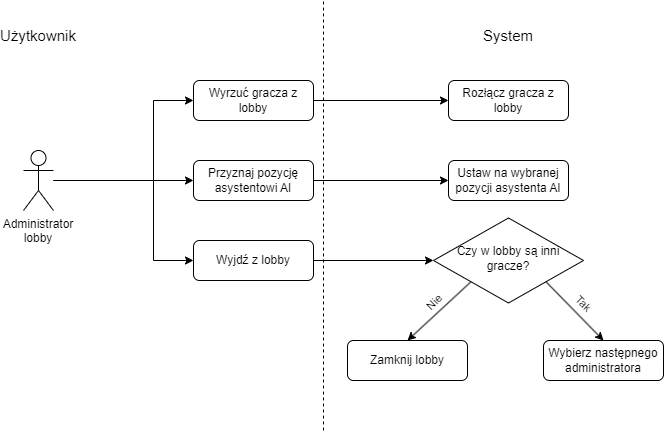
\includegraphics[width=0.9\textwidth]{img/schematy/manage_lobby.png}
  \caption{Schemat zarządzania lobby}
\end{figure}

\FloatBarrier


\subsubsection{Zgłoszenie gotowości}
Użytkownik po dołączeniu do lobby może zgłosić gotowość do rozgrywki poprzez
naciśnięcie przycisku "\textbf{Ready}". Kiedy wszyscy użytkownicy w lobby zgłoszą
gotowość, zaczyna się gra.


\subsection{Gra w brydża}

\subsubsection{Licytacja}

\begin{figure}[hbt!]
  \centering
  \includegraphics[width=0.9\textwidth]{img/schematy/bid.png}
  \caption{Schemat zgłoszenie odzywki}
\end{figure}

Na etapie początkowym gry, uczestnicy mają możliwość zgłaszania odzywek poprzez
aktywację przycisków odpowiadających ich wyborom. Mogą licytować kontrakty, pasować lub
deklarować kontrę i~rekontrę. Pierwszy licytujący jest losowo
wybranym graczem. Faza licytacji dobiega końca, gdy odzywka "pas" zostanie zagrana
trzy razy z rzędu.


\FloatBarrier


\subsubsection{Zagrywanie kart}

Po zakończeniu fazy licytacji, gracz podczas swojej kolejki może zagrać kartę,
przesuwając kursor na nią i klikając myszką. Dodatkowo, gracz będący partnerem dziadka
ma możliwość zagrywania kart w jego imieniu podczas jego tury.

\begin{figure}[hbt!]
  \centering
  \includegraphics[width=0.9\textwidth]{img/schematy/play_card.png}
  \caption{Schemat zagrania karty przez użytkownika}
\end{figure}

\FloatBarrier


\subsubsection{Zastąpienie gracza}
W przypadku, gdy jeden z graczy opuści grę, jego miejsce zostanie automatycznie
zajęte przez asystenta. Jednakże, jeśli wszyscy gracze kontrolowani przez ludzi
zdecydują się opuścić rozgrywkę, to zostanie ona zakończona.

% \subsection{Obserwowanie rozgrywek}

% Gdy jakaś rozgrywka w~brydża została rozpoczęta i~ma ona status
% publiczny, jest możliwe obejrzenie jej z~panelu \textbf{Watch}.
% Z~listy publicznych rozgrywek należy wybrać interesującą i~kliknąć
% ikonę oka. 
% \end{itemize}

% \begin{figure}[h]
%   \centering
%   \includegraphics[width=\textwidth]{example-image-a}
%   \caption{}
% \end{figure}

% \FloatBarrier


\section{Specyfikacja wymagań funkcjonalnych}

Aplikacja nie tylko powinna być dobrze zaprojektowana i~wygodna
w~użyciu, ale także funkcjonalna. Musi spełniać założone wymagania,
udostępniając odpowiednie funkcjonalności, żeby była przydatna dla
jej użytkowników. Nie da się używać wirtualnego asystenta do gry
w~brydża, jeśli brakuje w nim asystenta AI, czy w~ogóle elementu
rozgrywki. Bez spełnienia kluczowych wymagań funkcjonalnych,
aplikacja praktycznie nie istnieje. W~tym podrozdziale przedstawiamy
te wymagania.


\subsection{Logowanie i rejestracja nowych użytkowników}
Żeby uzyskać dostęp do funkcjonalności naszej aplikacji, potrzebne
jest posiadanie konta i bycie zalogowanym. Z~tego względu koniecznością
jest umożliwienie użytkownikom utworzenia konta, logowania się na
nie i~możliwość późniejszego wylogowania. Formularz rejestracji wymaga
podania adresu e-mail, nazwy użytkownika i~hasła. Logowanie odbywa się
poprzez wprowadzenie swojego adresu e-mail i~hasła.


\subsection{Lobby}
W celu rozegrania partii brydża przeciwko innym graczom bądź
przeciwnikom AI, gracz musi mieć możliwość utworzenia własnej
rozgrywki oraz dołączenia do istniejącej.

\subsubsection{Utworzenie/Dołączenie do lobby}
Utworzenie, jak i~dołączenie do lobby jest dostępne z~widoku głównego aplikacji. Dołączenie do lobby
odbywa się poprzez wprowadzenie identyfikatora gry. Po utworzeniu lobby użytkownik może
wysłać jego identyfikator innym graczom, zapraszając ich do dołączenia.

\subsubsection{Zarządzanie lobby}
Host powinien mieć możliwość dostosowania lobby według swoich preferencji przed
rozpoczęciem gry. Host ma prawo wyrzucić gracza z~lobby, zmienić jego pozycję lub przekazać
mu swoje uprawnienia. Dodatkowo, host powinien móc przydzielić wybrane pozycje
wirtualnym asystentom.


\subsection{Rozpoczęcie rozgrywki}
Kiedy wszystkie miejsca w lobby zostaną zajęte przez graczy, którzy zgłoszą gotowość do gry
lub część miejsc zostanie obsadzonych asystentami AI, rozgrywka zostaje rozpoczęta.
Wszyscy użytkownicy zostają przeniesieni do ekranu gry.


\subsection{Rozgrywka}
Głównym celem i~podstawową funkcjonalnością naszej aplikacji jest
rozgrywka w brydża. Każda runda zaczyna się od licytacji, po której
gracze wykładają karty zgodnie z~zasadami gry. Gra kończy się, kiedy
jedna z~par zdobędzie wystarczającą liczbę punktów. Po skończonej
rozgrywce użytkownikowi wyświetlany jest ekran z~wynikami.


\subsection{Wyświetlenie wyników}
Ważne jest, żeby gracze po skończeniu partii mogli zobaczyć
podsumowanie całej rozgrywki. Użytkownikowi wyświetlany jest ostateczny
wynik gry, a~także liczba zdobytych punktów przez jego zespół na
podstawie zdobytych lew. Dzięki temu gracze mogą dokładniej
przeanalizować rozegraną partię i~lepiej oceniać swoje możliwości
podczas licytacji w~przyszłych rozgrywkach.


\subsection{Opuszczenie rozgrywki}
Użytkownik może nie tylko wyjść z~lobby, ale także w~dowolnym momencie
opuścić rozgrywkę. W~takim przypadku miejsce gracza zastępuje
wirtualny asystent.



% TODO

\section{Specyfikacja wymagań niefunkcjonalnych}
W naszym projekcie aplikacji -- wirtualnego asystenta do gry w~brydża,
istotą jest zapewnienie nie tylko wszystkich potrzebnych wymagań
funkcjonalnych, ale także wygodnej i~przyjemnej rozgrywki oraz
korzystania z reszty funkcjonalności. Niewiele osób będzie chętnie
korzystać z~aplikacji, choćby miała ona wyjątkowo rozbudowane spektrum
funkcji, jeśli jej działanie będzie niestabilne i~pozbawione
intuicyjności. W~tym podrozdziale przedstawiamy wymagania
niefunkcjonalne aplikacji, które są równie ważne, jak zdefiniowane
wcześniej wymagania funkcjonalne.
\subsection{Dostępność}
Rozwijany przez nas wirtualny asystent do gry w~brydża jest aplikacją
webową. Dzięki temu będzie on dostępny zarówno dla użytkowników
Windows, MacOS, Linux, jak i~innych systemów operacyjnych posiadających
przeglądarkę wspierającą najnowsze standardy. Co więcej, starannie
zaprojektowane interfejsy użytkownika (UI) zostały dostosowane tak,
aby były wygodne i~funkcjonalne nawet na urządzeniach o~niewielkich
rozmiarach ekranu, umożliwiając płynne korzystanie z~aplikacji również
na urządzeniach mobilnych.
\subsection{Użyteczność}
Priorytetem naszej aplikacji jest zapewnienie łatwości obsługi
i~zrozumiałości. Niezwykle istotne jest, aby interfejs użytkownika
był intuicyjny, estetyczny i~nie zniechęcał potencjalnych użytkowników,
ani nie utrudniał korzystania z~aplikacji. Dlatego podczas projektowania
interfejsu użytkownika kierowaliśmy się zasadami dobrego UI/UX.
Stworzyliśmy minimalistyczny i~uporządkowany interfejs, który eliminuje
chaos i~zapewnia spójność na wszystkich podstronach aplikacji.
Wykorzystaliśmy ikony o~jednakowym znaczeniu na wszystkich stronach,
co ułatwia nawigację. Dodatkowo zastosowaliśmy stałą gamę starannie
dobranych kolorów dla elementów interfejsu, co pozwoliło nam utrzymać
spójny styl podczas projektowania kolejnych widoków. Aplikacja oferuje
tryb jasny i~ciemny, aby użytkownicy mogli wygodnie korzystać z~niej
w~zależności od preferencji lub pory dnia. Ponadto, wszystkie podstrony
są responsywne, co oznacza, że elementy interfejsu zachowują pełną
funkcjonalność, niezależnie od zmiany rozmiaru ekranu, na którym są
wyświetlane.
\subsection{Niezawodność}
Wirtualny asystent do gry w brydża tworzony jest z~myślą o~nauce
i~doskonaleniu umiejętności, ale także konkurencji i~wzajemnym
rozgrywkom pomiędzy graczami. Konieczne jest więc wprowadzenie logiki
gry z~największą dokładnością. Błędy w działaniu aplikacji podczas
rozgrywki mogłyby wpłynąć na wynik gry oraz wprowadzić nowych graczy
w~zakłopotanie, a~bardziej doświadczonych w~stan irytacji.
Niezwykle istotne jest również uniknięcie sytuacji, w~których
dochodziłoby do utraty połączenia lub braku synchronizacji pomiędzy
graczami. Takie incydenty mogą zrujnować całą rozgrywkę i~zdecydowanie
obniżyć wartość jednej z~kluczowych funkcjonalności aplikacji, jaką
jest możliwość rozgrywania partii między użytkownikami.
Pierwszym krokiem w~stronę niezawodności aplikacji było wybranie
odpowiednich technologii do jej realizacji. Next.js oraz FastAPI %%% TODO dowód?
to godne zaufania, popularne na całym świecie narzędzia do budowy
aplikacji webowych, a~usługa Google Firebase odciąża nas z~implementacji
funkcjonalności gromadzenia danych i~obsługi użytkowników od podstaw.
Mając odpowiedni stos technologiczny, przystąpiliśmy do implementacji
kolejnych funkcjonalności z~najwyższą starannością.

